\documentclass[a4paper,10pt,twoside,openany]{book}

\usepackage[lang=hebrew]{maths}
\usepackage{hebrewdoc}
\usepackage{stylish}
\usepackage{lipsum}
\let\bs\blacksquare

\title{סיכומי הרצאות לשיטות טופולוגיות בקומבינטוריקה (פיאונים קמורים) \\ \large{אביב 2021, הטכניון}}
\author{הרצאותיו של פרופ' רועי משולם \\ \large סוכמו על ידי אלעד צורני}
\date{\today}

\begin{document}
\frontmatter
\frontpage{polyhedron}{0.8\textwidth}{פוליהדרון קמור בשם \textenglish{Cuboctahedron-Rhombic Dodecahedron Compound}.}
\tableofcontents
\countlectures
\newpage

\chapter*{הקדמה}
\addcontentsline{toc}{chapter}{הקדמה} \markboth{הקדמה}{}

\section*{הבהרה}
\addcontentsline{toc}{section}{הבהרה} %\markboth{Technicalities}{}

סיכומי הרצאות אלו אינם רשמיים ולכן אין
\emph{כל הבטחה}
כי החומר המוקלד הינו בהתאמה כלשהי עם דרישות הקורס, או שהינו חסר טעויות.
\\
להיפך, ודאי ישנן טעויות בסיכום! אעריך אם הערות ותיקונים ישלחו אלי בכתובת דוא"ל
\textenglish{\href{mailto:tzorani.elad@gmail.com}{tzorani.elad@gmail.com}}.\\
אלעד צורני.

\section*{ספרות מומלצת.} %TODO edit
\addcontentsline{toc}{section}{ספרות מומלצת} %\markboth{Course Literature}{}

הספרות המומלצת עבור הקורס הינה כדלהלן.

\begin{english}
\begin{description}
\item[J. Matoušek, G. M. Ziegler:] Around Brouwer’s fixed point theorem

\item[J. Matoušek:] Using the Borsuk-Ulam Theorem

\item[D. Kozlov, R. Meshulam:] Around Helly's Theorem
\end{description}
\end{english}

\mainmatter

\chapter*{הקדמה}
\section{תוכן הקורס}

\subsection{פיאונים}

נדבר בקורס על קמירות ופיאונים.
פיאונים תלת־מימדיים רגולריים הם חמשת הגופים האפלטוניים: האוקטהדר, הקובציה, הסימפלקס, הדודקהדר והאיקוסהדר.
קיימות שאלות קשות ופתוחות על פיאונים. אנו נתרכז בדיון בשאלה שהייתה פתוחה עד לפני כחמישים שנה ועוסקת ומספרי הפיאות של פיאונים.

עבור פיאון
$P$
נסמן ב־%
$f_i\prs{P}$
את מספר הפיאות ה־%
$i$%
־מימדיות של
$P$.

במקרה של
$P$
הסימפלקס נקבל
\begin{align*}
\text{.} \prs{f_0, f_1, f_2} = \prs{4,6,4}
\end{align*}

נקרא ל־%
$\prs{f_0, \ldots, f_{d-1}}$
ה־%
$f$%
־וקטור ונסמנו
$f$.
במקרה של האוקטהדר נקבל
$f = \prs{6,12,8}$,
ובמקרה של הקוביה נקבל
$f\prs{8,12,6}$.

במקרה
$d = 2$,
פיאון הוא מצולע קמור ומתקיים
$f_0\prs{P} = f_1\prs{P}$.

במקרה
$d = 3$
נוסחאת אוילר אומרת
\[\text{.} f_0\prs{P} - f_1\prs{P} + f_2\prs{P} = 2\]

כמו כן, כל צלע משותפת לשתי פיאות. אם
$\abs{F}$
מספר הצלעות של פאה
$F$
נקבל
\begin{align*}
\text{.} 2 f_1\prs{P} = \sum_{F} \abs{F} \geq 3 \cdot f_2\prs{P}
\end{align*}
נציב זאת בנוסחאת אוילר ונקבל
\[2 = f_0\prs{P} - f_1\prs{P} + f_2\prs{P} \leq f_0\prs{P} - f_1\prs{P} + \frac{2}{3} f_1\prs{P} = f_0\prs{P} - \frac{1}{3} f_1\prs{P}\]
ואז
\[\text{.} f_1\prs{P} \leq 3 \prs{f_0\prs{P} - 2}\]
נקבל אז גם
\[\text{.} f_2\prs{P} \leq \frac{2}{3} f_1\prs{P} \leq 2 \prs{f_0\prs{P} - 2}\]
במקרה בו מספר הצלעות של פאה קבוע, נקבל שוויונים.

\subsection{בעיית החסם העליון לפיאונים}

יהי
$P$
פיאון
$d$%
־מימדי ב־%
$\mbb{R}^d$.
יהי
$f_0\prs{P}$
מספר קודקודיו.

\begin{question}
איך אפשר לחסום את
$f\prs{P} = \prs{f_1\prs{P}, \ldots, f_{d-1}\prs{P}}$?
\end{question}

\begin{question}
בהינתן
$n \ceq f_0\prs{P}$
מספר קודקודי
$P$,
איך אפשר לתאר את האפשרויות עבור
$f$?
\end{question}

\chapter{קמירות - גיאומטריה וקומבינטוריקה}

\section{הגדרות}

\begin{definition}[קטע בין נקודות]
עבור
$a,b \in \mbb{R}^d$
נגדיר את
\emph{הקטע בין
$a,b$}
להיות
\begin{align*}
\text{.} \brs{a,b} &= \set{\lambda a + \prs{1-\lambda} b}{\lambda \in \brs{0,1}}
\end{align*}
\end{definition}

\begin{definition}[צירוף קמור]
יהיו
$a_1, \ldots, a_k \in \mbb{R}^d$.
\emph{צירוף קמור של הם}
הוא
$\sum_{i \in [k]} \lambda_i a_i$
עבור
$\lambda_i \in \mbb{R}_{\geq 0}$
המקיימות
$\sum_i \lambda_i = 1$.
\end{definition}

\begin{definition}[קבוצה קמורה]
קבוצה
$K \subseteq \mbb{R}^d$
תקרא
\emph{קמורה}
אם לכל
$a,b \in K$
מתקיים
$\brs{a,b} \subseteq K$.
\end{definition}

\begin{definition}[תת־מרחב אפיני (ישרייה)]
$L \subseteq \mbb{R}^d$
נקרא
\emph{תת־מרחב אפיני}
אם
$L = v + U$
עבור
$U \leq \mbb{R}^d$
תת־מרחב ועבור
$v \in \mbb{R}^d$.
\end{definition}

\begin{definition}
אם
$L = v + U$
כנ"ל נגדיר
$\dim L \ceq \dim U$.
\end{definition}

\begin{definition}[על־מישור]
$L \subseteq \mbb{R}^d$
נקרא
\emph{על־מישור}
אם הוא תת־מרחב אפיני עם
$\codim L \ceq d - \dim L = 1$.
\end{definition}

\begin{definition}[צירוף אפיני]
צירוף אפיני של
$a_1, \ldots, a_k \in \mbb{R}^d$
הוא צירוף
$\sum_{i=1}^k \lambda_i a_i$
כאשר
$\sum_{i=1}^k \lambda_i = 1$.
\end{definition}

\begin{exercise}
בהינתן
$A \subseteq \mbb{R}^d$,
אוסף הצירופים האפיניים של איברי
$A$,
שנסמנו
$\mrm{aff}\prs{A}$,
הוא המרחב האפיני המינימלי שמכיל את
$A$.
\end{exercise}

\begin{definition}[קמור של קבוצה]
תהי
$A \subseteq \mbb{R}^d$.
\emph{הקמור של $A$},
שמסומן
$\conv\prs{A}$,
הוא הקבוצה הקמורה המינימלית שמכילה את
$A$.
\end{definition}

\begin{proposition}
מתקיים
\begin{align*}
\conv\prs{A} &= \bigcap_{\substack{K \supseteq A \\ \text{$K$ is convex}}} K
\\ \text{.} \hphantom{\conv\prs{A}} &= \set{\sum_{i \in [[k]} \lambda_i a_i}{\substack{a_1, \ldots, a_k \in A \\ \sum_{i \in [k]} \lambda_i = 1 \\ \lambda_i \geq 0}}
\end{align*}
\end{proposition}

\begin{proof}
תהי
\[\text{.} B \ceq \set{\sum_{i \in [[k]} \lambda_i a_i}{\substack{a_1, \ldots, a_k \in A \\ \sum_{i \in [k]} \lambda_i = 1 \\ \lambda_i \geq 0}}\]
אז
$B$
קמורה כי
\begin{align*}
\theta \sum_i \lambda_i a_i + \prs{1-\theta} \sum_i \mu_i a_i &= \sum_i \prs{\theta \lambda_i + \prs{1-\theta} \mu_i} a_i \\&=
\sum_i \theta \lambda_i + \prs{1-\theta} \mu_i
\end{align*}
וגם
\[\text{.} 1 = \theta + 1 - \theta = \theta \sum_i \lambda_i + \prs{1-\theta} \sum_i \mu_i\]

$B$
מינימלית כי כל קבוצה קמורה שמכילה את
$A$
צריכה להכיל צירופים קמורים של איברי
$A$.
\end{proof}

\section{משפטי הלי, קרתיאודורי ורדון}

\subsection{משפט הלי}

\begin{theorem}[הלי]
נסתכל על
$\mbb{R} = \mbb{R}^1$.
נניח ש־%
$I_1, \ldots, I_n$
קטעים ב־%
$\mbb{R}$
כך ש־%
$I_i \cap I_j \neq \ns$
לכל
$i,j \in [n]$.
אז
\[\text{.} \bigcap_{i \in [n]} I_i \neq \ns\]
\end{theorem}

\begin{proof}
נוכיח במקרה בו
$I_i = \brs{a_i, b_i}$.
המקרה הכללי דומה מאוד.

מההנחה, מתקיים
\[\text{.} c \ceq \max_{i \in [n]} \prs{a_i} \in \bigcap_{i \in [n]} I_i\]
\end{proof}

כעת ננסח את הגרסה המקורית של המשפט.

\begin{theorem}
יהיו
$K_1, \ldots, K_n$
קבוצות קמורות ב־%
$\mbb{R}^d$
המקיימות
\[\bigcap_{i \in I} K_i \neq \ns\]
לכל
$I \subseteq \brs{n}$
המקיימת
$\abs{I} \leq d + 1$.
אז
\[\text{.} \bigcap_{i \in [n]} K_i \neq \ns\]
\end{theorem}

הלי הוכיח את המשפט בתחילת המאה הקודמת.

%LECTURE 2

\subsection{משפטי ההפרדה}

\begin{definition}[]
$a_1, \ldots, a_k \in \mbb{R}^d$
יקראו
\emph{בלתי־תלויות אפינית}
אם
\[\text{.} \sum_{i \in [k]} \lambda_i a_i =0 \, \wedge \, \sum_{i \in [k]} \lambda_i = 0 \implies \prs{\lambda_1,\ldots, \lambda_k} = \prs{0, \ldots, 0}\]
\end{definition}

\begin{proposition}
התנאים הבאים שקולים עבור
$a_1, \ldots, a_k \in \mbb{R}^d$.

\begin{enumerate}
\item $a_1,\ldots,a_k$
בלתי־תלויות אפינית.
\item לכל
$i \in [k]$,
\[\text{.} a_i \notin \mrm{aff}\prs{a_1, \ldots, a_{i-1}, a_{i+1}, \ldots, a_k}\]
\item $\dim \mrm{aff}\prs{a_1, \ldots, a_k} = k-1$.
\item $a_1 - a_k, \ldots, a_{k-1}-a_k$
בלתי־תלויים לינארית.
\item \[\prs{a_1, 1}, \ldots, \prs{a_k, 1}\]
בלתי־תלויים לינארית.
\end{enumerate}
\end{proposition}

\begin{proof}
\begin{description}
\item[1 גורר 5:]
אם
$\prs{a_1,1}, \ldots, \prs{a_k,1}$
תלויים לינארית, ניתן לכתוב
\[\sum_{i \in [k]} \lambda_i \prs{a_1, 1} = 0\]
כאשר
$\prs{\lambda_1, \ldots, \lambda_k} \neq 0$.
אז
\begin{align*}
\sum_{i \in [k]} \lambda_i a_i = 0
\end{align*}
וגם
\begin{align*}
\text{.} \sum_{i \in [k]} \lambda_i = 0
\end{align*}
בסתירה לאי־תלות אפינית.
\item[5 גורר 1:]
בדומה לכיוון הקודם.
\item[1 גורר 2:]
נניח בשלילה שמתקיים
$a_k \in \mrm{aff}\prs{a_1, \ldots, a_{k-1}}$.
אז
\[a_k = \sum_{i \in [k-1]} \lambda_i a_i\]
וגם
\[\text{.} \sum_{i \in [k-1]} \lambda_i = 1\]
אז
\begin{align*}
\lambda_1 a_1 + \ldots + \lambda_{k-1} a_{k-1} - a_k = 0
\end{align*}
וסכום המקדמים הוא
\begin{align*}
\lambda_1 + \dots + \lambda_{k-1} - 1 = 1 - 1 = 0
\end{align*}
בסתירה לתלות האפינית של
$a_1, \ldots, a_k$.
\item[2 גורר 1:]
באופן דומה לכיוון הקודם.
\end{description}
\end{proof}

\begin{definition}
בהינתן
$u \in \mbb{R}^d \setminus \set{0}$
ו־%
$\alpha \in \mbb{R}$
נגדיר את העל־מישור
\begin{align*}
H_{u,\alpha} = \set{x \in \mbb{R}^d}{x \cdot u = \alpha}
\end{align*}
כאשר
\[\text{.} x \cdot u = \sum_{i \in [d]} x_i u_i\]
נגדיר גם את חצאי המרחב הסגורים
\begin{align*}
H_{u,\alpha}^+ \ceq \set{x \in \mbb{R}^d}{x \cdot u \geq u} \\
\text{.} H_{u,\alpha}^- \ceq \set{x \in \mbb{R}^d}{x \cdot u \leq u}
\end{align*}
\end{definition}

\begin{theorem}[משפט ההפרדה \textenglish{I}]
תהי
$K \subseteq \mbb{R}^d$
קמורה וסגורה ותהי
$p \in \mbb{R}^d \setminus K$.
קיימים
$u,\alpha$
כך ש־%
$p \in H_{u,\alpha}^+$
ו־%
$K \subseteq H_{u,\alpha}^-$.
\end{theorem}

\begin{proof}
תהי
$q \in K$
כך ש־%
\[\text{.} \norm{p - q} = \min \set{\norm{x-p}}{x \in K}\]
יהי
$H$
העל־מישור הניצב ל־%
$p-q$
ועובר דרך
$q$.
מפורשות,
$H = H_{p-q, \prs{p-q}\cdot q}$.
ראשית,
$p \in H^+_{p-q, \prs{p-q}\cdot q}$
כי
$p \cdot \prs{p-q} > \prs{p-q} \cdot q$
כי
$\norm{p-q}^2 > 0$.

תהי
$x \in K$.
לכל
$t \in \prs{0,1}$
מתקיים
\begin{align*}
\norm{p-q}^2 &\leq \norm{\prs{1-t}q + tx - p}^2
\\&= \norm{\prs{p-q} - t\prs{x-q}}^2
\\ \text{.} \hphantom{\norm{p-q}^2} &= \norm{p-q}^2 - 2t\prs{p-q}\cdot\prs{x-q} + t^2 \norm{x-q}^2
\end{align*}
לכן
\begin{align*}
\text{.} 2t \prs{p-q} \cdot \prs{x-q} \leq t^2 \norm{x-q}^2
\end{align*}
נצמצם
$t$
ונשאיף
$t \to \infty$.
נקבל
$\prs{p-q}\prs{x-q} \leq 0$
כלומר
$\prs{p-q} \cdot x \leq \prs{p-q} \cdot q$
ולכן
$x \in H^-_{p-q,\prs{p-q} \cdot q}$.
\end{proof}

\begin{theorem}[משפט ההפרדה \textenglish{II}]
תהי
$K$
קומפקטית קמורה ב־%
$\mbb{R}^d$
ותהי
$L$
קמורה וסגורה ב־%
$\mbb{R}^d$.
אם
$K \cap L = \ns$
קיים
$H_{u,\alpha}$
עבורו
$K \subseteq H_{u,\alpha}^+$
וגם
$L \subseteq H_{u,\alpha}^-$.
\end{theorem}

\begin{proof}
נעיין בקבוצה
$M = K - L$.
זאת קבוצה קמורה וסגורה:
אם
$x_i - y_i \xrightarrow{i\to\infty} z$
יש תת־סדרה
$x_{i_k} \xrightarrow{k\to\infty} x \in K$.
אז
$y_{i_k} \xrightarrow{k\to\infty} x-z$.
$L$
סגורה ולכן
$x-z \in L$.
אז
$z = x - \prs{x-z} \in M$.

$K \cap L = \ns$
לכן
$0 \notin M$,
ולכן אפשר להפריד בין
$0$
ל־%
$M$
על ידי על מישור
$H_{u,\alpha}$,
כלומר
\begin{align*}
0 &\in H_{u,\alpha}^+ \\
\text{.} M = K-L &\subseteq H_{u,\alpha}^-
\end{align*}
לכן
$0 = u \cdot 0 \geq 0$
ומאידך
$0 \geq \alpha \geq u \cdot \prs{x-y}$
לכל
$x \in K, y \in L$.
לכן
$u \cdot y \geq u \cdot x$
לכל
$x \in K, y \in L$.
ניקח
$\beta = \max_{x \in K} u \cdot x$.
אז לכל
$x \in K$
מתקיים
$u \cdot x \leq \beta$
ולכל
$y \in L$
מתקיים
$u \cdot y \geq \beta$.
\end{proof}

\subsection{משפטי קרתיאודורי ורדון}

\begin{theorem}[קרתיאודורי]\label{theorem:caratheodory}
תהי
$A \subseteq \mbb{R}^d$
ותהי
$p \in \mrm{conv}\prs{A}$.
קיימים
$a_1, \ldots, a_{d+1} \in A$
כך שמתקיים
$p \in \mrm{conv}\prs{a_1, \ldots, a_{d+1}}$.
\end{theorem}

\begin{proof}
יהי
$m \in \mbb{N}_+$
מינימלי כך שקיימים
$a_1, \ldots, a_m \in A$
עבורם
$p \in \mrm{conv}\prs{a_1, \ldots, a_m}$.
צריך להראות שמתקיים
$m \leq d+1$.
נניח בשלילה שמתקיים
$m \geq d+2$.
תהי
\[p = \sum_{i \in [m]} \lambda_i a_i\]
כאשר
$\sum_{i \in [m]} \lambda_i = 1$
וגם
$\lambda_i \geq 0$
לכל
$i \in [m]$.
נעיין ב־%
$m$
הוקטורים
$\prs{a_1, 1}, \ldots, \prs{a_m, 1} \in \mbb{R}^{d+1}$.
יש כאן
$d+2$
וקטורים, לכן קיימת תלות לינארית
\[\text{.} \sum_{i \in [m]} \alpha_i \prs{a_i,1} = 0\]
בפרט
\begin{align*}
\sum_{i \in [m]} \alpha_i = 0, \quad \sum_{i \in [m]} \alpha_i a_i = 0
\end{align*}
ובה"כ קיים
$\alpha_i > 0$.
תהי
\[\text{.} I = \set{i \in [m]}{\alpha_i > 0}\]
יהי
\[\text{.} \frac{\lambda_{i_0}}{\alpha_{i_0}} = \min\set{\frac{\lambda_i}{\alpha_i}}{i \in I}\]
אז
\begin{align*}
\sum_{i \in [m]} \prs{\lambda_i - \frac{\lambda_{i_0}}{\alpha_{i_0}} \cdot \alpha_i} a_i
&= \sum_{i \in [n]} \lambda_i a_i - \frac{\lambda_{i_0}}{\alpha_{i_0}} \sum_{i \in [m]} \alpha_i a_i
\\&= \sum_{i \in [m]} \lambda_i a_i
\\ \text{.} \hphantom{\sum_{i \in [m]} \prs{\lambda_i - \frac{\lambda_{i_0}}{\alpha_{i_0}} \cdot \alpha_i} a_i} &= p
\end{align*}

מצד שני, זהו צירוף קמור:
מתקיים
\begin{align*}
\text{.} \sum_{i\in[m]} \prs{\lambda_i - \frac{\lambda_{i_0}}{\alpha_{i_0}} \alpha_i}
&= \sum_{i \in [m]} \lambda_i - \frac{\lambda_{i_0}}{\alpha_{i_0}} \sum_{i \in [m]} \alpha_i = 0
\end{align*}
אם
$\alpha_i \geq 0$
מתקיים
\[ \lambda_i - \frac{\lambda_{i_0}}{\alpha_{i_0}} = \prs{\frac{\lambda_i}{\alpha_i} - \frac{\lambda_{i_0}}{\alpha_{i_0}}} \alpha_i \geq 0\]
ואם
$\alpha_i \leq 0$
מתקיים
\[\text{.} \lambda_i - \frac{\lambda_{i_0}}{\alpha_{i_0}} \alpha_i \geq \lambda_i > 0\]

 אבל, זהו צירוף של
$m-1$
איברים כי
\[\text{.} \lambda_{i_0} - \frac{\lambda_{i_0}}{\alpha_{i_0}} \alpha_{i_0} = 0\]
\end{proof}

במקרה
$d = 2$
משפט רדון אומר שאם
$A \subseteq \mbb{R}^2$
מקיימת
$4 \leq \abs{A}$,
ניתן לכתוב
$A = B \sqcup C$
כאשר
\[\text{.} \conv B \cap \conv C \neq \ns\]

\begin{theorem}[רדון]
אם
$a_1, \ldots, a_m \in \mbb{R}^d$
כאשר
$m \geq d + 2$,
יש חלוקה
$\set{1, \ldots, m} \supseteq I \sqcup J$
כך שמתקיים
\[\text{.} \conv \set{a_i}_{i \in I} \cap \conv \set{a_j}_{j \in J} \neq \ns\]
\end{theorem}

\begin{proof}
נעיין ב־%
$\prs{a_1, 1}, \ldots, \prs{a_m,1} \in \mbb{R}^{d+1}$.
מכיוון שהנחנו
$m \geq d+2$
קיימת תלות לינארית לא טריוויאלית
\[\text{.} \sum_{i \in [m]} \lambda_i \prs{a_i, 1} = 0\]
אז
\begin{align*}
\text{.} \sum_{i \in [m]} \lambda_i a_i = 0 , \quad \sum_{i \in [m]} \lambda_i = 0
\end{align*}
נסמן
\begin{align*}
I &\ceq \set{i \in [m]}{\lambda_i > 0} \\
J &\ceq \set{i \in [m]}{\lambda_i < 0}
\end{align*}
וגם
\[\text{.} \lambda \ceq \sum_{i \in I} \lambda_i = - \sum_{j \in J} \lambda_j\]
אז
\begin{align*}
\text{.} \sum_{i \in I} \frac{\lambda_i}{\lambda} = -\sum_{j \in J} \frac{\lambda_j}{\lambda} = 1
\end{align*}
כמו כן,
\begin{align*}
\sum_{i \in I} \lambda_i a_i = - \sum_{j \in J} \lambda_j a_j
\end{align*}
לכן
\begin{align*}
\text{.} \sum_{i \in I} \frac{\lambda_i}{\lambda} a_i = - \sum_{j \in J} \frac{\lambda_j}{\lambda} a_j \in \conv\prs{a_i}_{i \in I} \cap \conv\prs{a_j}_{j \in J}
\end{align*}
\end{proof}

\begin{remark}
$d+2$
הוא המספר המינימלי שמבטיח תוצאה כזאת, מפני שאם ניקח
$a_1, \ldots, a_{d+1}$
כוקטורים בלתי־תלויים אפינית, לכל נקודה ב־%
$\conv\prs{a_1, \ldots, a_{d+1}}$
יש הצגה יחידה כצירוף קמור של
$a_1, \ldots, a_{d+1}$.
למשל עבור
$0, e_1, \ldots, e_d$
אין חלוקת רדון.
\end{remark}

\subsection{משפט הלי הכללי}

\begin{theorem}[הלי]
תהי
$\mcal{K}$
משפחה סופית של קבוצות קמורות ב־%
$\mbb{R}^d$
כך שלכל
$\mcal{G} \subseteq \mcal{K}$
המקיימת
$\abs{G} \leq d+1$
מתקיים
\[\text{.} \bigcap_{K \in \mcal{G}} K \neq \ns\]
אז
\[\text{.} \bigcap_{K \in \mcal{K}} K \neq \ns\]
\end{theorem}

\begin{proof}
נניח בשלילה שלא כל הקבוצות ב־%
$\mcal{K}$
נחתכות. נבחר
$m \in \mbb{N}_+$
מינימלי כך שקיימות
$K_1, \ldots, K_m \in \mcal{K}$
עבורן
\begin{align*}
\text{.} \bigcap_{i \in [m]} K_i = \ns
\end{align*}
נרצה להראות שגם
\[\text{,} \bigcap_{i \in [m]} K_i \neq \ns\]
מה שיתן סתירה.

מההנחה נובע
$m \geq d+2$.
לכל
$j \in [m]$
נבחר
\[\text{.} x_j \in \bigcap_{i \in [m] \setminus \set{j}} K_i\]
לפי משפט רדון, יש חלוקה
$\brs{m} = J_1 \sqcup J_2$
עבורה
\[\text{.} \conv\prs{x_j}_{j \in J_1} \cap \conv\prs{x_j}_{j \in J_2} \neq \ns\]
תהי
$p \in \conv\prs{x_j}_{j \in J_1} \cap \conv\prs{x_j}_{j \in J_2}$,
נראה שבעצם
$p \in \bigcap_{i \in [m]} K_i$.

יהי
$i \in [m]$.
נניח כי
$i \in J_2$
ויהי
$j \in J_1$.
אז
\begin{align*}
\text{.} x_j \in \bigcap_{t \in [m] \setminus \set{j}} K_t \subseteq \bigcap_{t \in J_2} K_t \subseteq K_i
\end{align*}
אז
\begin{align*}
p \in \conv\prs{x_j}_{j \in J_1} \subseteq K_i
\end{align*}
מקמירות.
מאידך, אם
$i \in J_1, j \in J_2$
נקבל
\begin{align*}
\text{.} x_j \in \bigcap_{t \in [m] \setminus \set{j}} K_t \subseteq \bigcap_{t \in J_1} K_t \subseteq K_i
\end{align*}
אז
\begin{align*}
\text{.} p \in \conv\prs{x_j}_{j \in J_2} \subseteq K_i
\end{align*}
בסך הכל,
$p \in \bigcap_{i \in [m]} K_i$,
בסתירה למינימליות
$m$.
\end{proof}

\subsection{שימושים למשפט הלי}

תהיינה קבוצות סופיות
$A,B \subseteq \mbb{R}^d$.
נרצה לשאול מתי יש
$H_{u,\alpha}$
עבורו
$A \in \mrm{int} H_{u,\alpha}^+, B \subseteq \mrm{int} H_{u,\alpha}^-$.
המשפט הבא מתאר איך ניתן לבדוק זאת.

\begin{theorem}[קירכנברגר]
אם לכל
$A_0 \subseteq A, B_0 \subseteq B$
כך שמתקיים
$\abs{A_0} + \abs{B_0} \leq d+2$
אפשר להפריד בין
$A_0, B_0$
על ידי על מישור, אפשר להפריד גם את
$A,B$
על ידי על מישור.
\end{theorem}

\begin{proof}
לכל
$a \in A$
נגדיר
\[\text{.} K_a \ceq \set{\prs{u,\alpha} \in \mbb{R}^d \times \mbb{R}}{u \cdot a > \alpha}\]
נוכל לחשוב על זה כעל חצי־המישור
\[\text{.} \set{\prs{u,\alpha} \in \mbb{R}^{d+1}}{\prs{u,\alpha} \cdot \prs{a,-1} > 0}\]
לכל
$b \in B$
נגדיר באופן דומה
\begin{align*}
L_b &\ceq \set{\prs{v,\beta} \in \mbb{R}^d \times \mbb{R}}{v \cdot b < \beta}
\\ \text{.} \hphantom{L_b} &= \set{\prs{v,\beta} \in \mbb{R}^{d+1}}{\prs{v,\beta}\prs{b,-1} < 0} 
\end{align*}
$K_a, L_b$
קמורות כפנים של חצי־מישור.
מתקיים
\[\bigcap_{a \in A} K_a \neq \ns\]
כי
$\prs{0,-1}$
נמצא בחיתוך.
באופן דומה
\[\prs{0,1} \in \bigcap_{b \in B} L_b\]
אז גם חיתוך זה אינו ריק.

נניח כי
$\abs{A_0} + \abs{B_0} \leq d+2$
ונטען כי
\begin{align*}
\text{.} \bigcap_{a \in A_0} K_a \cap \bigcap_{b \in B_0} L_b \neq \ns
\end{align*}
לפי ההנחה, קיים על מישור
$H_{u,\alpha}$
שמפריד בין
$A_0, B_0$.
אז
$a \cdot u > \alpha$
וגם
$b \cdot u < \alpha$
לכל
$a \in A_0, b \in B_0$.
כלומר,
$\prs{u,\alpha} \in K_a$
לכל
$a \in A_0$
וגם
$\prs{u,\alpha} \in L_b$
לכל
$b \in B_0$.

לפי משפט הלי נובע כי
\[\text{.} \bigcap_{a \in A} K_a \cap \bigcap_{b \in B} L_b \neq \ns\]
ניקח
$\prs{u,\alpha}$
בחיתוך ונקבל
\begin{align*}
A &\subseteq \mrm{int} H_{u,\alpha}^+ \\
\text{.} B &\subseteq \mrm{int} H_{u,\alpha}^-
\end{align*}
\end{proof}

\begin{theorem}[רדו]
תהי
$C \subseteq \mbb{R}^d$
חסומה ומדידה לבג.
קיימת נקודה
$p \in \mbb{R}^d$
כך שלכל על מישור
$H_{u,\alpha}$
דרך
$p$
מתקיים
\[\text{.} \mu\prs{H_{u,\alpha}^+ \cap C} \geq \frac{1}{d+1} \mu\prs{C}\]
\end{theorem}

\begin{proof}
ראשית נעיר שמשפט הלי גורר שאם
$\prs{K_{\alpha}}_{\alpha \in \mcal{A}}$
קמורות וקומפקטיות ב־%
$\mbb{R}^d$
כך שכל
$d+1$
מהן נחתכות אז
$\bigcap_{\alpha \in \mcal{A}} K_\alpha \neq \ns$.
זה נובע מכך שאם כל תת־אוסף סופי של קבוצות קומפקטיות נחתך, כולן נחתכות.

יהי
$0<\eps<\frac{1}{d+1}$.
לכל
$u \in S^{d-1}$
ולכל
$t \in \mbb{R}$
נעיין בחיתוך
$C \cap H_{u,t}^+$.
מתקיים
\begin{align*}
\lim_{t\to -\infty} \mu\prs{C \cap H_{u,t}^+} &= \mu\prs{C} \\
\text{.} \lim_{t\to\infty} \mu\prs{C \cap H_{u,t}^+} &= 0
\end{align*}
לכן מרציפות המידה יש
$\lambda\prs{u} \in \mbb{R}$
כך שמתקיים
\[\text{.} \mu\prs{C \cap H_{u,\lambda\prs{u}}^+} = \prs{\frac{d}{d+1} + \eps} \mu\prs{C} \]

יהי
$B$
כדור שמכיל את
$C$.
אז
$K_u \ceq H_{u,\lambda\prs{u}}^+ \cap C$
קמורה.
נראה שאם
$u_1, \ldots, u_{d+1} \in S^{d-1}$
אז
\[ \text{.} K_{u_1} \cap \ldots \cap K_{u_{d+1}} \neq \ns\]
לכל
$i \in [d+1]$
מתקיים
\begin{align*}
\prs{\frac{d}{d+1} + \eps} \mu\prs{C} \leq \mu\prs{H^+_{u_i, \lambda\prs{u_i}} \cap C}
\end{align*}
ולכן
\begin{align*}
\text{.} \prs{\frac{1}{d+1} - \eps} \mu\prs{A} \geq \mu\prs{H^-_{u_i, \lambda\prs{u_i} \cap C}}
\end{align*}
אם
$\bigcap_{i \in [d+1]} K_{u_i} = \ns$
אז
\begin{align*}
\bigcap_{i \in [d+1]} H^+_{u_i, \lambda\prs{u_i}} \cap B = \ns
\end{align*}
ולכן
\begin{align*}
\text{.} \bigcup_{i \in [d+1]} B \cap H^-_{u_i, \lambda\prs{u_i}} = B \cap \bigcup_{i \in [d+1]} H^-_{u_i, \lambda\prs{u_i}} = B
\end{align*}
אז
\begin{align*}
C = \bigcup_{i \in [d+1]} C \cap H_{u_i, \lambda\prs{u_i}}^-
\end{align*}
בסתירה לכך שמתקיים
\begin{align*}
\text{.} \sum_{i \in \brs{d+1}} \mu\prs{C \cap H_{u_i, \lambda\prs{u_i}}^-} \leq \prs{d+1} \prs{\frac{1}{d+1} - \eps} \mu\prs{C} < \mu\prs{C}
\end{align*}

לכן
$\bigcap_{i \in [d+1]} K_{u_i} \neq \ns$
לכל
$u_1, \ldots, u_{d+1} \in S^d$,
ולפי הלי
$\bigcap_{u \in S^{d-1}} K_u \neq \ns$.
ניקח
$p \in \bigcap_{u \in S^{d-1}} K_u$.
אם נעביר על מישור
$H_{u,\alpha}$
שכיוונו
$u \in S^{d-1}$
דרך
$p$,
אז
\begin{align*}
\text{.} \prs{H_{u,\alpha}^- \cap C} \geq \prs{\frac{1}{d+1} - \eps} \mu\prs{C}
\end{align*}
נקבל
$H_{u,\alpha}^+ \subseteq H_{u,\lambda\prs{u}}^+$
ואז
\begin{align*}
\mu\prs{H_{u,\alpha}^+ \cap C} &\leq \mu\prs{H_{u,\lambda\prs{u}}^+ \cap C}
\\ \text{.} \hphantom{\mu\prs{H_{u,\alpha}^+ \cap C}} &= \prs{\frac{d}{d+1} + \eps} \mu\prs{C}
\end{align*}
לכן
\[H_{u,\lambda\prs{u}}^- \cap C \subseteq H_{u,\alpha}^- \cap C\]
ו־%
\begin{align*}
\text{.} \prs{\frac{1}{d+1} - \eps} \mu\prs{C} = \mu\prs{H_{u,\lambda\prs{u}} \cap C} \leq \mu\prs{H_{u,\alpha}^- \cap C}
\end{align*}

עתה
$p \ceq \lim_{z\to\infty} \frac{p_z}{z}$
תקיים את הדרוש.
\end{proof}

%LECTURE 13.4.2021

למשפט הלי יש גרסה שקולה עבור משפחה לאו דווקא סופית של קבוצות קומפקטיות.

\begin{theorem}[הלי]
תהי
$\mcal{K}$
משפחה של קבוצות קומפקטיות קמורות ב־%
$\mbb{R}^d$.
אם כל
$d+1$
קבוצות מ־%
$\mcal{K}$
נחתכות, כל הקבוצות נחתכות.
\end{theorem}

תהי
$A \subseteq \mbb{R}^d$
ונניח שמתקיים
$\mrm{diam}\prs{A} = 1$.
נרצה לחשוב מהו הרדיוס המינימלי של כדור
$B\prs{p,r}$
המכיל את
$A$.
במקרה
$d = 1$
אפשר להסתכל על
$A$
כמוכלת בקטע מאורך
$1$
ואז
$r_1 = \frac{1}{2}$
הרדיוס המינימלי.
במקרה
$d=2$
נוכל להסתכל על הדוגמה של משולש שווה צלעות.
אז הרדיוס המינימלי הוא
\[\text{.} r_2 = \frac{\frac{1}{2}}{\cos\prs{\frac{\pi}{6}}} = \frac{1}{\sqrt{3}}\]

נעיין במקרה הכללי ברדיוס המינימלי עבור הסימפלקס ה־%
$d$
מימדי הרגולרי.
יהי
\[\text{.} H \ceq \set{x \in \mbb{R}^{d+1}}{\sum_{i \in [d+1]} x_i = \frac{1}{\sqrt{2}}} \cong \mbb{R}^d\]
ב־%
$H$
נעיין בסימפלקס שקודקודיו הם
$\frac{e_i}{\sqrt{2}} \in H$
עבור
$i \in [d+1]$.
מתקיים
\[\text{.} \abs{\frac{e_i}{\sqrt{2}} - \frac{e_j}{\sqrt{2}}} = \prs{\prs{\frac{1}{\sqrt{2}}}^2 + \prs{\frac{1}{\sqrt{2}}}^2}^{\frac{1}{2}} = 1\]
מרכז הכובד של הסימפלקס הוא
\[\text{.} p = \frac{1}{d+1} \sum_{i \in [d+1]} \frac{e_i}{\sqrt{2}}\]
אז
\begin{align*}
\frac{e_j}{\sqrt{2}} - p &= \frac{1}{\sqrt{2}} \prs{- \frac{e_1}{d+1} + \ldots + \frac{-e_{j-1}}{d+1} + \frac{d}{d+1} e_j + \frac{-e_{j+1}}{d+1} + \ldots + \frac{-e_{d+1}}{d+1}}
\end{align*}
ואז
\begin{align*}
\abs{\frac{e_j}{\sqrt{2}} - p}^2 &= \frac{1}{2} \prs{\prs{\frac{1}{d+1}}^2 + \ldots + \prs{\frac{1}{d+1}}^2 + \prs{\frac{d}{d+1}}^2}
\\&= \frac{1}{2} \prs{\frac{d}{d+1}^2 + \frac{d^2}{\prs{d+1}^2}}
\\ \text{.} \hphantom{\abs{\frac{e_j}{\sqrt{2}} - p}^2} &= \frac{d}{2 \prs{d+1}}
\end{align*}
נקבל כי
$r_d \ceq \sqrt{\frac{d}{2\prs{d+1}}}$
רדיוס הכדור החוסם של הסימפלקס הרגולרי באורך צלע
$1$
ב־%
$\mbb{R}^d$.

משפט יונג אומר לנו בעצם מה הרדיוס עבור קבוצה
$A$
כללית.

\begin{theorem}[יונג]
תהי
$A \subseteq \mbb{R}^d$
מקוטר
$1$.
קיימת
$p \in \mbb{R}^d$
עבורה
$A \subseteq B\prs{p,r_d}$
כאשר
$r_d \ceq \sqrt{\frac{d}{2\prs{d+1}}}$.
\end{theorem}

\begin{proof}
נעיין באוסף הכדורים
$\set{B\prs{a, r_d}}_{a \in A}$.
די להראות כי
$\bigcap_{a \in A} B\prs{a, r_d} \neq \ns$.

ממשפט הלי נובע שדי להראות שאם
$a_1, \ldots, a_{d+1} \in A$
אז
$\bigcap_{i \in [d+1]} B\prs{a_i, r_d} \neq \ns$.
כלומר, די להראות שכל
$d+1$
נקודות מ־%
$A$
מוכלות בכדור ברדיוס
$r_d$.

יהי
$B\prs{p,r}$
כדור עם רדיוס מינימלי המכיל את
$a_1, \ldots, a_{d+1}$.
בלי הגבלת הכלליות יהיו
$a_1, \ldots, a_m$
הנקודות הנמצאות על שפת
$B\prs{p,r}$.

נטען כי
$p \in \conv\set{a_1, \ldots, a_m}$.
אחרת,
$p \notin K \ceq \conv\set{a_1, \ldots, a_m}$
ולכן יש על־מישור
$H$
שמפריד בין
$K,p$.
אם נזיז את מרכז הכדור מעט לכיוון הניצב ל־%
$h$
נקבל שכל $a_1, \ldots, a_{d+1}$ בפנים של כדור מרדיוס
$r$,
בסתירה למינימליות.

נראה עתה כי
$r \leq r_d$
ונניח בלי הגבלת הכלליות כי
$p = 0$.
אז יש
$\lambda \geq 0$
עבורם
\begin{align*}
\sum_{i \in [m]} \lambda_i a_i &= 0 \\
\text{.} \hphantom{la} \sum_{i \in [m]} \lambda_i &= 1
\end{align*}
נקבל
\begin{align*}
1 &\geq \abs{a_i - a_j}^2
\\&= \abs{a_i}^2 + \abs{a_j}^2 - 2 a_i \cdot a_j
\\&= r^2 + r^2 - 2 a_i \cdot a_j
\end{align*}
ולכן
$2 a_i \cdot a_j \geq 2r^2 - 1$.
אז
\begin{align*}
0 &= \abs{\sum_{i \in [m]} \lambda_i a_i}^2
\\&= \sum_{i \in [m]} \lambda_i^2 \abs{a_i}^2 + 2 \sum_{1 \leq 1 < j \leq m} \lambda_i \lambda_j a_i \cdot a_j
\\&\geq \sum_{i \in [m]} \lambda_i^2 r^2 + \sum_{1 \leq i < j \leq m} \lambda_i \lambda_j
\\&= r^2 \prs{\sum_{i \in [m]} \lambda_i^2 + 2 \sum_{1 \leq i < j \leq m} \lambda_i \lambda_j} - \sum_{1 \leq i < j \leq m} \lambda_i \lambda_j
\\&= r^2 \prs{\sum_{i \in [m]} \lambda_i}^2 - \sum_{1 \leq i < j \leq m} \lambda_i \lambda_j 
\\ \text{.} \hphantom{0} &= r^2 - \sum_{1 \leq i < j \leq m} \lambda_i \lambda_j 
\end{align*}
נקבל
\[\text{.} r^2 \leq \sum_{1 \leq i < j \leq m} \lambda_i \lambda_j \leq \max_{\substack{x_i \geq 0 \\ \sum x_i = 1}} \prs{\sum_{1 \leq i < j \leq m} x_i x_j}\]

אם נראה שהמקסימום מתקבל כאשר כל ה־%
$x_i$
בביטוי האחרון שווים נקבל
\[\binom{m}{2} \frac{1}{m^2} = \frac{m\prs{m-1}}{2m^2} = \frac{m-1}{2m} \leq \frac{d}{2d+1}\]
ואז
$r \leq \sqrt{\frac{d}{2\prs{d+1}}} = r_d$.
אכן,
\begin{align*}
\sum_{1 \leq i < j \leq m} x_i x_j &= \frac{1}{2} \prs{\prs{\sum_{i \in [m]} x_i}^2 - \sum_{i \in [m]} x_i^2}
\\&= \frac{1}{2} \prs{1 - \sum_{i \in [m]} x_i^2}
\end{align*}
כאשר
\[\frac{1}{m} \sum_{i \in [m]} x_i^2 \geq \prs{\frac{1}{m} \sum_{i \in [m]} x_i}^2\]
מקמירות של
$x \mapsto x^2$.
אז
$\sum_{i \in [m]} x_i^2 \geq \frac{1}{m}$
ונקבל כי
\[\text{.} \sum_{1 \leq i < j \leq m} x_i x_j = \frac{1}{2} \prs{1 - \sum_{i \in [m]} x_i^2} \leq \frac{1}{2} \prs{1 - \frac{1}{m}} = \frac{1}{2} \frac{m-1}{m}\]
\end{proof}

\section{גרסאות מודרניות של משפטי קרתיאודורי והלי}

\subsection{משפט קרתיאודורי הצבעוני}

\begin{theorem}[קרתיאודורי]
יהיו
$A_1, \ldots, A_{d+1} \subseteq \mbb{R}^d$
ותהי
$p \in \bigcap_{i \in [d+1]} \conv\prs{A_i}$.
אז יש נקודות
$a_i \in A_i$
לכל
$i \in [d+1]$
עבורן
$p \in \conv\prs{a_1, \ldots, a_{d+1}}$.
\end{theorem}

\begin{proof}
בלי הגבלת הכלליות נניח כי
$\abs{A_i} < \infty$
(לפי \ref{theorem:caratheodory} אפשר לקחת
$\abs{A_i} \leq d+1$).
יהיו
$a_1 \in A_1, \ldots, a_{d+1} \in A_{d+1}$
עבורן
$\rho \ceq d\prs{p, \conv\set{a_1, \ldots, a_{d+1}}}$
מינימלי.
עלינו להראות שמתקיים
$\rho = 0$.
נניח בשלילה ש־%
$\rho > 0$.
תהי
$q \in \conv\set{a_i}{i \in [d+1]}$
כך ש־%
\[\text{.} \abs{p-q} = \min\set{\norm{x-p}}{x \in \conv\set{a_i}{i \in [d+1]}}\]
אז
\[\conv\set{a_i}{i \in \brs{d+1}} \subseteq H_{p-q, \prs{p-q} \cdot q}^- \eqqcolon H\]
כפי שראינו בחישוב קודם.
אז
\[\text{.} q \in H\]
ממשפט
\ref{theorem:caratheodory}
נובע ש־%
$q$
בקמור של
$d$
נקודות מבין
$a_1, \ldots, a_{d+1}$,
ובלי הגבלת הכלליות נניח כי
$q \in \conv\set{a_1, \ldots, a_d}$.

אנו יודעים כי
$p \in A_{d+1}$.
לכן
$A_{d+1} \nsubseteq H$.
לכן קיימת נקודה
$a_{d+1} \in A_{d+1} \setminus H$.
אז
\[\text{.} \prs{a_{d+1}' - q} \cdot \prs{p-q} > 0\]
נראה שמתקיים
\[\text{.} d\prs{p, \conv\set{a_1, \ldots, a_d, a_{d+1}'}} < \rho\]
נעיין בנקודה
$\prs{1-t}q + t a_{d+1}'$
עבור
$t$
קטן.
מתקיים
\begin{align*}
\abs{p - \prs{\prs{1-t} q + ta_{d+1}'}}^2 &= \abs{\prs{p-q} - t \prs{a_{d+1}' - q}}^2
\\ \text{.} \hphantom{\abs{p - \prs{\prs{1-t} q + ta_{d+1}'}}^2} &= \abs{p-q}^2 - 2t \prs{p-q} \cdot \prs{a_{d+1}' - q} + t^2 \abs{a_{d+1}' - q}^2
\end{align*}
כעת, אם
$t \in \prs{0,1}$
קטן מספיק
אז
\[2t \prs{p-q} \cdot \prs{a_{d+1}' - q} > t \abs{a_{d+1}' - q}\]
ולכן
\[\abs{p - \prs{\prs{1-t} q + ta_{d+1}'}}^2 < \rho^2\]
בסתירה למינימליות של
$\set{a_1, \ldots, a_{d+1}}$.
\end{proof}

\subsection{מסקנות מקרתיאודורי צבעוני}

\begin{theorem}[הלי צבעוני] \label{theorem:colourful-helly}
תהיינה
$\mcal{K}_1, \ldots, \mcal{K}_{d+1}$
משפחות של קבוצות קמורות ב־%
$\mbb{R}^d$.
נניח שלכל
\[\prs{K_1, \ldots, K_{d+1}} \in \prod_{i \in [d+1]} \mcal{K}_i\]
מתקיים
\[\text{.} \bigcap_{i \in [d+1]} K_i \neq \ns\]
אז יש
$j \in [d+1]$
כך שכל הקבוצות ב־%
$\mcal{K}_j$
נחתכות.
\end{theorem}

\begin{theorem}[טברברג]
תהי
$A \subseteq \mbb{R}^d$
מגודל
$\prs{d+1}\prs{k-1} + 1$.
אז אפשר לכתוב
$A = \bigsqcup_{i \in [k]} A_k$
כאשר
\[\text{.} \bigcap_{i \in [k]} \conv\prs{A_i} \neq \ns\]
\end{theorem}

\subsection{קרתיאודורי עבור חרוטים}

\begin{definition}
עבור
$A \subseteq \mbb{R}^{d+1}$
נגדיר
את ה־%
\emph{\textenglish{positive span} של $A$}
על ידי
\begin{align*}
\text{.} \mrm{pos}\prs{A} \ceq \set{\sum_{i \in [m]} \lambda_i a_i}{a_i \in A, \, \lambda_i \geq 0}
\end{align*}
\end{definition}

\begin{definition}
קבוצה
$C \subseteq \mbb{R}^{d+1}$
נקראת
\emph{חרוט קמור שקודקודו
$0$}
אם
$C$
קמורה ולכל
$c \in C$
גם
$\lambda c \in C$
לכל
$\lambda \geq 0$.
\end{definition}

\begin{remark}
לכל
$A \subseteq \mbb{R}^{d+1}$
הקבוצה
$\mrm{pos}\prs{A}$
היא חרוט קמור ב־%
$\mbb{R}^{d+1}$.
\end{remark}

\begin{theorem}[קריתיאודורי עבור קמור חיובי]
תהי
$A \subseteq \mbb{R}^{d+1}$
ותהי
$p \in \mrm{pos}\prs{A}$.
אזי יש
$A_0 \subseteq A$
עם
$\abs{A_0} \leq d+1$
כך שמתקיים
$p \in \mrm{pos}\prs{A_0}$.
\end{theorem}

\begin{proof}
בדיוק כמו בהוכחת משפט קרתיאודורי, נבחר
$A_0 = \set{u_1, \ldots, u_n} \subseteq A$
מינימלית עבורה
$p \in \mrm{pos}\set{u_1, \ldots, u_n}$.
נכתוב
\[p = \sum_{i \in [n]} \lambda_i u_i\]
עם
$\lambda_i \geq 0$,
ונראה כי
$d+1 \geq n$.
אחרת,
$n \geq d+2$
ולכן יש צירוף לינארי
\[\sum_{i \in [n]} \mu_i u_i = 0\]
שאינו טריוויאלי.
תהי
\[\theta \ceq \min \set{\frac{\lambda_i}{\mu_i}}{\mu_i > 0}\]
(בלי הגבלת הכלליות קיימים
$\mu_i > 0$)
ויהי
$i_0 \in [n]$
עבורו
$\theta = \frac{\lambda_{i_0}}{\mu_{i_0}}$.
אז
\begin{align*}
p &= \sum_{i \in [n]} \lambda_i u_i
\\&= \sum_{i \in [n]} \prs{\lambda_i - \theta \mu_i} u_i
\\&= \sum_{i \neq i_0} \prs{\lambda_i - \theta \mu_i} u_i + \cancelto{0}{\prs{\lambda_{i_0} - \frac{\lambda_{i_0}}{\mu_{i_0}} \mu_{i_0}}} u_{i_0}
\end{align*}
וקיבלנו את
$p$
כיצירוף חיובי של פחות מה־%
$u_i$.
\end{proof}

\begin{theorem}[קרתיאודורי החיובי עבור קמור חיובי]
תהיינה
$A_1, \ldots, A_{d+1} \subseteq \mbb{R}^{d+1}$
ותהי
$p \in \bigcap_{i \in [d+1]} \mrm{pos}\prs{A_i}$.
אז יש
$a_i \in A_{i}$
לכל
$i \in [d+1]$
עבורן
\[\text{.} p \in \mrm{pos}\set{a_1, \ldots, a_{d+1}}\]
\end{theorem}

\begin{lemma}\label{lemma:pos-conditions}
נניח כי
$u_1, \ldots, u_m \in \mbb{R}^{d+1}$.
נגיד שהן מקיימות את תנאי
1
אם
$\prs{\vec{0}, -1} \in \mrm{pos}\set{u_1, \ldots, u_m}$.
יהיו
$H_{u_i, 0}$
על־מישורים הניצבים ל־%
$u_i$
ונסתכל על חצאי המרחבים
$H_{u_i, 0}^+$.
נגיד שה־%
$u_i$
מקיימות את תנאי 2 אם
\[\text{.} \bigcap_{i \in [m]} H_{u_i, 0}^+ \cap \mbb{R}^d \times \set{1} = \ns\]
נטען כי תנאים 1 ו־2 שקולים.
\end{lemma}

\begin{proof}
\begin{itemize}
\item נניח שמתקיים תנאי 1 ויהיו
$\lambda_i \geq 0$
עבורן
\[\text{.} \prs{\vec{0}, -1} = \sum_{i \in [m]} \lambda_i u_i\]
נניח כי
$z \in \bigcap_{i \in [m]} H_{u_i, 0}^+$
ונראה כי הקואורדינטה האחרונה של
$z$
אי־חיובית.
אכן,
\begin{align*}
-z_{d+1} &= \prs{\vec{0}, -1} \cdot z
\\&= \sum_{i \in [m]} \lambda_i \prs{u_i \cdot z}
\\&\geq 0
\end{align*}
כלומר
$z_{d+1} \leq 0$
ובפרט
$z \notin \mbb{R}^d \times \set{1}$.
\item נניח שתנאי 1 אינו מתקיים ונראה כי תנאי 2 אינו מתקיים.
נניח כי
\[\text{.} \prs{\vec{0}, -1} \notin C \ceq \mrm{pos}\set{u_1, \ldots, u_m}\]
נפריד את
$C$
מ־%
$\prs{\vec{0}, -1}$
על ידי על מישור
$H_{w,\alpha}$.
כלומר,
\[\text{.} \forall z \in C \colon \prs{0,-1} \cdot w < \alpha \leq z \cdot w\]
מתקיים
$0 \in C$
לכן
$\alpha \leq 0 \cdot w = 0$
ונקבל
$\alpha \leq 0$.
אם עבור
$i \in [m]$
כלשהו מתקיים
$u_i \cdot w < 0$
נקבל
\[\lim_{\lambda \to \infty} \prs{\lambda u_i} \cdot w = -\infty < \alpha\]
בסתירה כי
$\lambda u_i \in C$
לכל
$\lambda \geq 0$.

לכן
$\alpha \leq 0$
וגם
$u_i \cdot w \geq 0$
לכל
$i \in [m]$.
נקבל
\[-w_{d+1} = \prs{\vec{0}, -1} \cdot w < \alpha \leq 0\]
ולכן
$w_{d+1} > 0$.
אז
$w \in H_{u_i, 0}^+$
ואז
\[\text{.} \frac{w}{w_{d+1}} \in \bigcap_{i \in [m]} H_{u_i, 0}^+ \cap \mbb{R}^d \times \set{1}\]
לכן תנאי 2 אינו מתקיים.
\end{itemize}
\end{proof}

\begin{definition}[פיאון קמור]
\emph{פיאון קמור}
הוא קמור של מספר סופי של נקודות.
\end{definition}

\begin{definition}[עצב]
בהינתן
$K = \set{K_1, \ldots, K_m}$
משפחה של קבוצות קמורות ב־%
$\mbb{R}^d$
נגדיר את
\emph{העצב \textenglish{(nerve)}
של
$\mcal{K}$}
על ידי
\[\text{.} N\prs{\mcal{K}} \ceq \set{I \subseteq \brs{m}}{\bigcap_{i \in I} K_i \neq \ns}\]
\end{definition}

\begin{remark}
העצב של
$\mcal{K}$
מתאר את החיתוכים של קבוצות ב־%
$\mcal{K}$.
זה קומפלקס סימפליציאלי: אם
$\sigma \in N\prs{\mcal{K}}$
וגם
$\tau \subseteq \sigma$
אז
$\tau \in N\prs{\mcal{K}}$.
העצב של
$N\prs{\mcal{K}}$
שקול הומוטופית ל־%
$\bigcup_{K \in \mcal{K}} K$,
אבל נדון בכך בהמשך.
\end{remark}

\begin{theorem}[הלי במונחי העצב]
תהי
$\mcal{K} = \set{K_1, \ldots, K_m}$
משפחת קבוצות קמורות ב־%
$\mbb{R}^d$.
אם
$N\prs{\mcal{K}}$
מכיל את כל
$\sigma \subseteq \brs{m}$
המקיימת
$\abs{\sigma} \leq d+1$
אז
$N\prs{K} = \mcal{P}\prs{\brs{m}}$
אוסף כל התת־קבוצות של
$\brs{m}$.
\end{theorem}

\begin{proposition}\label{proposition:polytopes-nerve}
יהיו
$K_1, \ldots, K_m$
קבוצות קמורות ב־%
$\mbb{R}^d$
ותהי
$\mcal{K} \ceq \set{K_1, \ldots, K_m}$.
אז קיימים פיאונים
$P_1, \ldots, P_m$
עבורם
$P_i \subseteq K_i$
לכל
$i \in [m]$
וגם
\[M\prs{P} = N\prs{\mcal{K}}\]
כאשר
$\mcal{P} \ceq \set{P_1, \ldots, P_m}$.
\end{proposition}

\begin{remark}
שאלה מעניינת היא האם אפשר לאפיין את העצבים האפשריים של אוספי קבוצות קמורות ב־%
$\mbb{R}^d$.
בעוד זאת שאלה קשה באופן כללי, יש איפיון במקרה
$d = 1$.
למשל, אנו יודעים שאת הגרף באיור
\ref{figure:1}
אי אפשר לקבל כעצב ב־%
$\mbb{R}$.
\begin{figure}
\centering
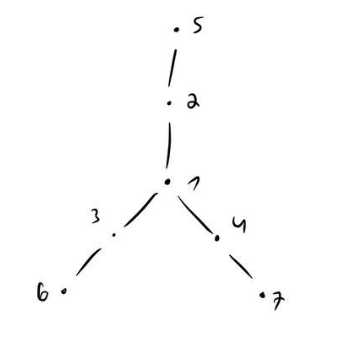
\includegraphics[scale=0.4]{sources/1}
\caption{קומפלקס שלא ניתן לקבל כעצב של קבוצת קטעים במישור.}
\label{figure:1}
\end{figure}

יהי
$\mcal{K} = \set{I_i}{i \in [7]}$
אוסף של שבעה קטעים ב־%
$\mbb{R}$.
במקרה זה,
$I_6$
חותך את
$I_3$
שחותך את
$I_1$,
אבל
$I_1$
לא חותך את
$I_6$
אז נקבל קטעים כמו באיור
\ref{figure:2}.
\begin{figure}
\centering
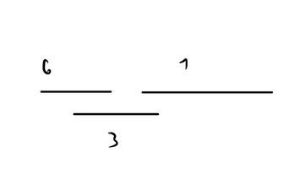
\includegraphics[scale=0.4]{sources/2}
\caption{}
\label{figure:2}
\end{figure}
כעת
$I_2$
חותך את
$I_1$
ואת
$I_5$
שזר ל־%
$I_1$
לכן נקבל קטעים כמו באיור
\ref{figure:3}.
\begin{figure}
\centering
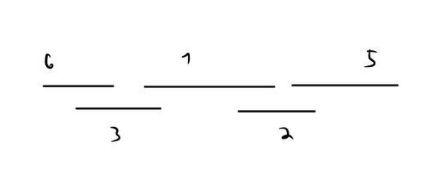
\includegraphics[scale=0.4]{sources/3}
\caption{}
\label{figure:3}
\end{figure}
אז
$I_4$
שחותך את
$I_1$
חייב להיות בין
$I_3, I_2$
אבל אז
$I_4 \subseteq I_!$
ולכן
$I_7$
שחותך את
$I_4$
חותך גם את
$I_1$.
ראו איור
\ref{figure:4}.
\begin{figure}
\centering
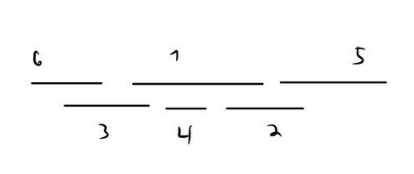
\includegraphics[scale=0.4]{sources/4}
\caption{}
\label{figure:4}
\end{figure}
\end{remark}

\begin{proof}
לכל
$\sigma \in N\prs{\mcal{K}}$
נבחר
$p_\sigma \in \bigcap_{i \in \sigma} K_i$.
נגדיר
\[\text{.} P_i \ceq \conv\set{p_\sigma}{i \in \sigma \in N\prs{\mcal{K}}}\]
נשים לב שאם
$i \in \sigma$
אז
$p_\sigma \in K_i$.
לכן
$P_i \subseteq K_i$.
לכן
$N\prs{\mcal{P}} \subseteq N\prs{\mcal{K}}$.
מאידך, אם
$\sigma \in N\prs{\mcal{K}}$
אז
$p_\sigma \in \bigcap_{i \in \sigma} P_i$
ולכן
$\sigma \in N\prs{\mcal{P}}$.
\end{proof}

\begin{corollary}\label{corollary:disjoint_halfplanes}
תהיינה
$K_1, \ldots, K_m$
קומפקטיות קמורות עבורן
$\bigcap_{i \in [m]} K_i = \ns$.
אזי קיימים חצאי מרחבים
$D_1, \ldots, D_m$
כך שמתקיים
$K_i \subseteq D_i$
לכל
$i \in [m]$,
וגם
$\bigcap_{i \in [m]} D_i = \ns$.
\end{corollary}

\begin{proof}
נוכיח באינדוקציה על
$\ell$
שקיימים
$D_1, \ldots, D_\ell$
עבורם
$K_i \subseteq D_i$
וגם
\[\text{.} D_1 \cap \ldots \cap D_\ell \cap K_{\ell + 1} \cap \ldots \cap K_m = \ns\]
נניח שהוכחנו עבור
$\ell < m$
ונוכיח עבור
$\ell+1$
(זה כולל את מקרה הבסיס).
אז
\begin{align*}
D_1 \cap \ldots \cap D_\ell \cap K_{\ell + 1} \cap \ldots \cap K_m = \ns
\end{align*}
כלומר
\begin{align*}
K_{\ell+1} \cap \prs{D_1 \cap \ldots \cap D_{\ell} \cap K_{\ell + 2} \cap \ldots \cap K_m} = \ns
\end{align*}
ולכן קיים
$H_{u,\alpha}^+$
עבורו
$K_{\ell+1} \subseteq H_{\u,\alpha}^+$
וגם
\[\text{.} D_1 \cap \ldots \cap D_\ell \cap K_{\ell+2} \cap \ldots \cap K_m \subseteq \mrm{int}H_{u,\alpha}^-\]
כלומר,
\[\text{.} D_1 \cap \ldots \cap D_\ell \cap K_{\ell+2} \cap \ldots \cap K_m \cap H_{u,\alpha}^+ = \ns\]
ניקח
$D_{\ell+1} \ceq H_{\u,\alpha}^+$.
\end{proof}

\begin{proof}[\ref{theorem:colourful-helly}]
בלי הגבלת הכלליות, מטענה
\ref{proposition:polytopes-nerve}
אפשר להניח ש־%
$K_{i,j}$
קומפקטיות לכל
$K_{i,j} \in \mcal{K}_i$.

לפי
\ref{corollary:disjoint_halfplanes}
קיימים חצאי מרחבים
$D_{i,j}$
כך ש־%
$K_{i,j} \subseteq D_{i,j}$
לכל
$K_{i,j} \in \mcal{K}_i$
וכך שמתקיים
$\bigcap_{j} D_{i,j} = \ns$.
נציג
\[\text{.} D_{i,j} = H_{u_{i,j}, \alpha_{i,j}}^+ = \set{v \in \mbb{R}^d}{v \cdot u_{i,j} \geq \alpha_{i,j}}\]
יהי
$w_{i,j} = \prs{u_{i,j}, -\alpha_{i,j}} \in \mbb{R}^{d+1}$.

נשים לב שמתקיים
\[\bigcap_j H_{w_{i,j}, 0}^+ \cap \prs{\mbb{R}^d \times \set{1}} = \ns\]
אם
$v = \prs{v', v_{d+1}}$
בחיתוך הנ"ל אז
$w_{i,j} \cdot \prs{v', v_{d+1}} \geq 0$
ומצד שני
$v_{d+1} = 1$.
אז
\begin{align*}
v' \cdot u_{i,j} + \prs{-\alpha_{i,j}} \cdot 1 \geq 0
\end{align*}
ולכן
$v' \cdot u_{i,j} \geq \alpha_{i,j}$
לכל
$j$.
אז
$v' \in D_{i,j}$
לכל
$j$,
בסתירה לכך שמתקיים
\[\text{.} \bigcap_j D_{i,j} = \ns\]
לכן, לפי
\ref{lemma:pos-conditions}
מתקיים
\[\prs{\vec{0}, -1} \in \mrm{pos}\set{w_{i,j}}_j\]
לכל
$i \in [d+1]$.
לפי קרתיאודורי הצבעוני עבור
\textenglish{pos}
קיימת בחירה
$w_{1, j_1}, w_{2,j_2}, \ldots, w_{d+1, j_{d+1}}$
כך שמתקיים
\[\text{.} \prs{\vec{0},-1} \in \mrm{pos}\set{w_{i,j_i}}_{i \in [d+1]}\]

לפי
\ref{lemma:pos-conditions}
נקבל כי
\[\text{.} \bigcap_{i \in \brs{d+1}} H_{w_{i,j_i},0}^+ \cap \prs{\mbb{R}^d \times \set{1}} = \ns\]
אז
\[\bigcap_{i \in [d+1]} K_{i, j_i} \subseteq \bigcap_{i \in [d+1]} D_{i, j_i} = f\bigcap_{i \in \brs{d+1}} H_{u_{i,j_i, \alpha_{i, j_i}}}^+ = \ns\]
כיוון שאם
$z \in \bigcap_{i \in [d]} H_{u_{i,j_i}, \alpha_{i,j_i}}^+$
אז
$z \cdot u_{i,j_i} \geq \alpha_{i,j_i}$
לכל
$i$
ואז
\begin{align*}
\prs{z,1} \cdot w_{i,j_i} &= \prs{z,1} \cdot \prs{u_{i,j_i}, -\alpha_{i,j_i}}
\\&= z \cdot u_{i, j_i} - \alpha_{i,j_i} > 0
\end{align*}
ונקבל כי
\[\prs{z,1} \in \bigcap_{i \in [d+1]} H_{w_{i,j_i}}^+ \cap \prs{\mbb{R}^d \times \set{1}}\]
בסתירה לביטוי קודם.
קיבלנו
\[\bigcap_{i \in [d+1]} K_{i, j_i} = \ns\]
בסתירה להנחה.
\end{proof}

\begin{theorem}[רדון]
תהיינה
$u_1, \ldots, u_{d+2} \in \mbb{R}^d$.
קיימת חלוקה
$\brs{d+2} = I_1 \sqcup I_2$
עבורה
\begin{align*}
\text{.} \conv\set{u_i}_{i \in I_1} \cap \conv\set{u_i}_{i \in I_2} = \ns
\end{align*}
\end{theorem}

נשאל מה מספר הנקודות המינימלי
$m$
כך שלכל
$u_1, \ldots, u_m \in \mbb{R}^2$
תהיה חלוקה
$\brs{m} = I_1 \sqcup I_2 \sqcup I_3$
עבורה
\[\text{.} \bigcap_{j \in [3]} \conv\set{u_i}_{i \in I_j} \neq \ns\]

\begin{theorem}[טברברג] \label{theorem:tverberg}
אם
$u_1, \ldots, u_m \in \mbb{R}^d$
וגם
$m \geq \prs{d+1}\prs{k-1} + 1$
אז יש חלוקה
$\brs{m} = \bigsqcup_{j \in [k]} I_j$
וגם
\[\text{.} \bigcap_{j \in [k]} \conv\set{u_i}_{i \in I_j} \neq \ns\]
\end{theorem}

\begin{remark}
על ידי הסתכלות על
$d+1$
קבוצות בגודל
$k-1$
 של נקודות קרובות (או שוות זאת לזאת, לא הנחנו שה־%
$u_i$
שונות)
  ב־%
$\mbb{R}^d$
אפשר לראות שהחסם התחתון במשפט טברברג אופטימלי, כיוון שבמקרה זה אין חלוקת
$k$%
־טברברג.
\end{remark}

%lecture 27.4.2021

בהוכחת משפט טברברג נרצה לעבוד במרחב
$\prs{k-1}\prs{d+1}$%
־מימדי.
נזכיר כי
$M_{k \times \ell}\prs{\mbb{R}} \cong \mbb{R}^k \tensor \mbb{R}^\ell$
מרחב ממימד
$k\ell$.
בהינתן
$u \in \mbb{R}^k, v \in \mbb{R}^\ell$
נגדיר
\[\text{.} u \tensor v \ceq u v^T = \pmat{u_1 v_1 & & \cdots & & u_\ell v_\ell \\ & & & & \\ \vdots & & & & \vdots \\ & & & & \\ u_k v_1 & & \cdots & & u_k v_\ell}\]

\begin{proposition}
נניח כי
$v_1, \ldots, v_k \in \mbb{R}^{k-1}$
מקיימים
\[\sum_{i \in [k]} v_i = 0\]
ושזאת התלות היחידה ביניהם.
למשל אפשר לקחת
$v_1, \ldots, v_{k-1}$
בסיס ל־%
$\mbb{R}^{k-1}$
ו־%
$v_k = -\prs{v_1 + \ldots + v_{k-1}}$
(זה בעצם המקרה הכללי).
נניח גם כי
$u_1, \ldots, u_k \in \mbb{R}^{N}$
מקיימים
\[\text{.} \sum_{i \in [k]} u_i \tensor v_i = 0 \in \mbb{R}^N \tensor \mbb{R}^{\prs{k-1}} \cong M_{N \times \prs{k-1}}\]
אז
$u_i = u_j$
לכל
$i,j \in [k]$.
\end{proposition}

\begin{remark}
ברור שאם
$u_i = u_j$
לכל
$i,j \in [k]$
אז
\[\text{.} \sum_{i \in \brs{k}} u_i \tensor v_i = u \tensor \sum_{i \in \brs{k}} v_i = u \tensor 0 = 0\]
\end{remark}

\begin{proof}
יהי
$z \in \mbb{R}^N$.
מתקיים
\begin{align*}
0 &= z^T \cdot \prs{\sum_{i \in [k]} u_i v_i^T} = \sum_{i \in [k]} \prs{z^T \cdot u_i} \cdot v_i^T
\end{align*}
לכן
$z^T \cdot u_i = z^T \cdot u_j$
לכל
$i,j \in [k]$.
זה נכון לכל
$z \in \mbb{R}^N$
לכן
$z^T \prs{u_i - u_j} = 0$
לכל
$z \in \mbb{R}^n$
ולכן
$u_i = u_j$.
\end{proof}

\begin{proof}[\ref{theorem:tverberg}]
על ידי הוספת רכיב לכל
$u_i$
אפשר להניח כי
$u_1, \ldots, u_m \in \mbb{R}^{d+1}$
וגם ש־%
$u_i \cdot \1 = 1$
כאשר
$\1 = \pmat{1 \\ 1 \\ \vdots \\ 1 \\ 1} \in \mbb{R}^{d+1}$.
יהיו
$v_1, \ldots, v_k \in \mbb{R}^{k-1}$
עבורם
$\sum_{i \in [k]} v_i = 0$
וזאת התלות היחידה ביניהם.
נשתמש בקרתיאודורי הצבעוני עבור
$\mbb{R}^{\prs{d+1}\prs{k-1}} \cong M_{\prs{d+1} \times \prs{k-1}}\prs{\mbb{R}}$.
לכל
$i \in [m]$
תהי
\[\text{.} A_i = \set{u_i \tensor v_j}{j \in [k]} \subseteq \mbb{R}^{\prs{d+1}\prs{k-1}}\]

מתקיים
$0 \in \bigcap_{i \in [m]} \conv\prs{A_i}$
כי
\[\text{.} 0 = u_i \tensor 0 = u_i \tensor \prs{\frac{1}{k} \sum_{j \in [k]} v_j} = \frac{1}{k} \sum_{j \in [k]} u_i \tensor v_j\]
לפי קרתיאודורי הצבעוני, לכל
$i \in \brs{m}$
קיים
$j_i \in [k]$
כך שמתקיים
\[\text{.} 0 \in \conv\set{u_i \tensor v_{j_i}}{i \in [m]}\]
אז יש
$\lambda_i \geq 0$
המקיימות
\begin{align*}
\sum_{i \in [m]} \lambda_i &= 1 \\
\text{.} \sum_{i \in [m]} \lambda_i \prs{u_i \tensor v_{j_i}} &= 0
\end{align*}
אבל אם נסמן
\[I_j \ceq \set{i \in [m]}{j_i = j}\]
נקבל
\begin{align*}
\text{.}  \sum_{j \in [k]} \prs{\sum_{i \in I_j} \lambda_i u_i} \tensor v_j &= \sum_{i \in [m]} \lambda_i \prs{u_i \tensor v_{j_i}} = 0
\end{align*}
לפי הטענה, קיים
$w \in \mbb{R}^d$
כך שלכל
$j \in [k]$
מתקיים
\[\text{.} w = \sum_{i \in I_j} \lambda_i u_i\]
אז
\[w \cdot \1 = \sum_{i \in I_j} \lambda_i \cdot \prs{u_i \cdot \1} = \sum_{i \in I_j} \lambda_i\]
ולכן
\begin{align*}
\frac{w}{w \cdot \1} &= \sum_{i \in I_j} \frac{\lambda_i}{w \cdot \1} \cdot u_i
\\&= \sum_{i \in I_j} \frac{\lambda_i}{\sum_{t \in I_j} \lambda_t} u_i
\\&\in \conv\set{u_i}_{i \in I_j}
\end{align*}
כנדרש.
\end{proof}

\subsection{משפט הנקודה הכבדה של
\textenglish{Barany}}

\begin{theorem}[\text{Barany}]
לכל
$d \geq 1$
יש קבוע
$C_d > 0$
כך שלכל
$u_1, \ldots, u_n \in \mbb{R}^d$
יש
$\mcal{F} \subseteq \binom{\brs{n}}{d+1}$
עבורה
$\abs{\mcal{F}} > C_d \binom{n}{d+1}$
וכך שקיימת
\[\text{.} p \in \bigcap_{F \in \mcal{F}} \conv\set{u_i}{i \in F}\]
\end{theorem}

\begin{proof}
נגדיר את
$k$
להיות השלם המקסימלי עבורו
$\prs{k-1}\prs{d+1} + 1 \leq n$.
כלומר,
$k = \floor{\frac{n-1}{d+1}} + 1$.

נניח כי
$k \geq d+1$.
לפי משפט
\ref{theorem:tverberg}
נחלק את
$\brs{n}$
לקבוצות זרות
$I_1, \ldots, I_k$
כך שיש
\[\text{.} p \in \bigcap_{j \in [k]} \conv\set{u_i}_{i \in I_j}\]
לכל בחירה
$\alpha_1 < \ldots < \alpha_{d+1}$
של איברים ב־%
$\brs{k}$
מתקיים
\[\text{.} p \in \bigcap_{t \in \brs{d+1}} \conv\set{u_i}{i \in I_{\alpha_t}}\]
לפי קרתיאודורי הצבעוני יש
$d+1$
נקודות, אחת מכל
$\set{u_i}_{i \in I_{\alpha_t}}$
כך ש־%
$p$
בקמור שלהן.
נסמן את קבוצת האינדקסים של נקודות אלו ב־%
$F_{\alpha}$
כאשר
$\alpha = \prs{\alpha_1, \ldots, \alpha_{d+1}}$.
אם
$\alpha \neq \beta$
נקבל
$F_\alpha \neq F_\beta$
ולכן
\[\mcal{F} \ceq \set{F_{\alpha}}{1 \leq \alpha_1 < \ldots < \alpha_{d+1} \leq k}\]
קבוצה מגודל
$\binom{k}{d+1}$.
אז
\begin{align*}
\abs{\mcal{F}}
&=
\binom{k}{d+1}
\\&=
\binom{\floor{\frac{n-1}{d+1}} + 1}{d+1}
\\&\geq
\binom{\floor{\frac{n-1}{d+1}}}{d+1}
\\&\geq
\frac{\prs{\floor{\frac{n-1}{d+1}} - d + 1}^{d+1}}{\prs{d+1}!}
\\&\geq \frac{\prs{\frac{n-1}{d+1} - d}^{d+1}}{\prs{d+1}!}
\\&= \frac{\prs{n-d^2 - d - 1}^{d+1}}{\prs{d+1}^{d+1} \prs{d+1}!}
\\&\geq \frac{n^{d+1} - \prs{d+1}\prs{d^2 + d + 1} n^d}{\prs{d+1}^{d+1} \prs{d+1}1}
\\&= \frac{1}{\prs{d+1}^{d+1}} \brs{\frac{n^{d+1}}{\prs{d+1}!} - \frac{\prs{d+1}\prs{d^2 + d + 1}}{\prs{d+1}!} n^d}
\\&\geq \frac{1}{\prs{d+1}^{d+1}} \prs{\binom{n}{d+1} - \lambda_d n^d}
\\&\geq \frac{1}{2 \prs{d+1}^{d+1}} \binom{n}{d+1}
\end{align*}
עבור קבוע
$\lambda_d$
וכאשר האי־שוויון האחרון נכון עבור
$n$
גדול מספיק.
נבחר
$C_d = \frac{1}{2 \prs{d+1}^{d+1}}$.
\end{proof}

\begin{remark}
בהינתן
$d$
אפשר לשאול מה הסופרמום
$\theta_d$
של ערכים
$\theta$
עבורם לכל
$n$
נקודות ב־%
$\mbb{R}^d$
יש
$p$
נקודות בלפחות
$\theta \cdot \binom{n}{d+1}$
מהסימפלקסים על ידי הנקודות.

עבור
$d \in \set{1,2}$
ידועים הערכים של
$\theta_d$.
עבור
$d > 2$
זאת בעיה פתוחה.
\end{remark}

%TODO 28.4

\subsection{רשתות
$\eps$
חלשות}

תהי
$\mcal{K}$
משפחה של קבוצות מדידות במרחב הסתברות
$\prs{\Omega, B, \mu}$.
נעיין בקבוצה
\[\text{.} A_{\eps} \ceq \set{K \in \mcal{K}}{\mu\prs{K} \geq \eps}\]
נרצה למצוא
$S \subseteq \Omega$
מגודל מינימלי כך ש־%
$S \cap K \neq \ns$
לכל
$K \in A_\eps$.

\begin{example}
יהי
$\Omega = \mbb{R}$
עם מידת הסתברות
$\mu$
המתוארת באופן הבא.
יהיו
$u_1 \leq \ldots \leq u_n$
נקודות ב־%
$\mbb{R}$.
נגדיר
\begin{align*}
\mu \ceq \frac{1}{n} \sum_{i \in [n]} \delta_{u_i}
\end{align*}
כאשר
$\delta_{u_i}$
מידת דיראק של
$u_i$.
נשאל האם יש
$S \subseteq \Omega$
סופית מגודל קטן מ־%
$f\prs{\eps}$
עבור
$f\prs{\eps}$
קבוע כלשהו התלוי באפסילון וכך שכל
$K \in A_\eps$
חותכת את
$S$.

תהי
\[\text{.} S = \set{u_{i \floor{\eps n}}}{i \in \floor{\frac{1}{\eps}}}\]
אז לכל קטע
$K$
עם
$\mu\prs{K} \geq \eps$
מתקיים
$K \cap S \neq \ns$.
אבל גם
$\abs{S} \leq \floor{\frac{1}{\eps}}$.
\end{example}

\begin{theorem}
תהא
$\mu$
מידת הסתברות דיסקרטית על
$\mbb{R}^d$
הנקבעת על ידי
$\set{u_i}_{i \in [n]} \subseteq \mbb{R}^d$
ו־%
\[\text{.} \mu\prs{A} = \frac{1}{n} \abs{\set{i}{u_i \in A}}\]
תהא
$\mcal{K}$
משפחת הקבוצות הקמורות ב־%
$\mbb{R}^d$.
אז יש
$S \subseteq \mbb{R}^d$
עם
$\abs{S} \leq \lambda_d \cdot \prs{\frac{1}{\eps}}^{d+1}$
עבורה
$S \cap K \neq \ns$
לכל
$K$
המקיימת
$\mu\prs{K} \geq \eps$.
\end{theorem}

\begin{proof}
לכל
$K \in \mcal{K}$
עבורה
$\mu\prs{K} \geq \eps$
תהא
$I_K \ceq \set{i}{u_i \in K}$.
אז
$\abs{I_k} \geq \eps n$.
לפי משפט הנקודה הכבדה, יש
$\mcal{F}_K \subseteq \binom{I_k}{d+1}$
עם
\[\abs{\mcal{F}_K} \geq c_d \cdot \binom{\abs{I_k}}{d+1} \geq c_d \binom{\eps n}{d+1}\]
וכך שקיימת
\[\text{.} p_K \in \bigcap_{F \in \mcal{F}_K} \conv\set{u_i}_{i \in F}\]
נבחר משפחה מקסימלית
$K_1, \ldots, K_r$
מתוך ה־%
$K \in \mcal{K}$
המקיימות
$\mu\prs{K} \geq \eps$
כך ש־%
$\mcal{F}_{K_1}, \ldots, \mcal{F}_{K_r}$
זרות בזוגות.

אז
\begin{enumerate}
\item $S = \ceq \set{p_{K_1}, \ldots, p_{K_r}}$
מקיימת
$S \cap K \neq \ns$
לכל
$K \in \mcal{K}$
עבורה
$\mu\prs{K} \geq \eps$:

תהא
$K$
כזאת. אז ממקסימליות
$K_1, \ldots, K_r$
נובע שקיים
$i \in \brs{r}$
עבורו
$\mcal{F}_K \cap \mcal{F}_{K_i} \neq \ns$.
אז קיימת
$F \in \mcal{F}_K \cap \mcal{F}_{K_i}$.
כעת,
$\set{u_j}{j \in F} \subseteq K \cap K_i$.
לכן
\[\text{.} p_{K_i} \in \conv\set{u_j}{j \in F} \subseteq K\]

\item נותר להראות ש־%
$r$
תלוי ב־%
$\eps$
בלבד.
מתקיים
\begin{align*}
\bigsqcup_{i \in [r]} \mcal{F}_{K_i} \subseteq \binom{\brs{n}}{d+1}
\end{align*}
לכן
\[\text{.} \sum_{i \in [r]} \abs{\mcal{F}_{K_i}} \\leq \binom{n}{d+1}\]
אבל
\[r \cdot c_d \binom{\floor{\eps} n}{d+1} \leq \sum_{i \in [r]} \abs{\mcal{F}_{K_i}} \leq \binom{n}{d+1}\]
ולכן
\begin{align*}
r &\leq \frac{\binom{n}{d+1}}{c_d \binom{\floor{\eps}n}{d+1}}
\\&\leq \frac{\frac{n^{d+1}}{\prs{d+1}!}}c_d \frac{\prs{\prs{\eps n  - d}^{d+1}}}{\prs{d+1}!}
\\&= \frac{1}{c_d} \prs{\frac{n}{\eps n - d}}^{d+1}
\\ \text{.} \hphantom{r} &\xrightarrow{n\to\infty} \frac{1}{c_d} \prs{\frac{1}{\eps}}^{d+1}
\end{align*}
\end{enumerate}
\end{proof}

\chapter{פיאונים}

%TODO

\begin{comment}

\end{comment}

\backmatter
\end{document}